\documentclass[12pt]{article}

\usepackage{sbc-template}

\usepackage{graphicx,url}

\usepackage[brazil]{babel}   
%\usepackage[latin1]{inputenc}  
\usepackage[utf8]{inputenc}  
% UTF-8 encoding is recommended by ShareLaTex

     
\sloppy

\title{Instructions for Authors of SBC Conferences\\ Papers and Abstracts}

\author{Luciana P. Nedel\inst{1}, Rafael H. Bordini\inst{2}, Flávio Rech
  Wagner\inst{1}, Jomi F. Hübner\inst{3} }


\address{Instituto de Informática -- Universidade Federal do Rio Grande do Sul
  (UFRGS)\\
  Caixa Postal 15.064 -- 91.501-970 -- Porto Alegre -- RS -- Brazil
\nextinstitute
  Department of Computer Science -- University of Durham\\
  Durham, U.K.
\nextinstitute
  Departamento de Sistemas e Computação\\
  Universidade Regional de Blumenal (FURB) -- Blumenau, SC -- Brazil
  \email{\{nedel,flavio\}@inf.ufrgs.br, R.Bordini@durham.ac.uk,
  jomi@inf.furb.br}
}

\begin{document} 

\maketitle

\begin{abstract}
  This meta-paper describes the style to be used in articles and short papers
  for SBC conferences. For papers in English, you should add just an abstract
  while for the papers in Portuguese, we also ask for an abstract in
  Portuguese (``resumo''). In both cases, abstracts should not have more than
  10 lines and must be in the first page of the paper.
\end{abstract}
     
\begin{resumo} 
  Este meta-artigo descreve o estilo a ser usado na confecção de artigos e
  resumos de artigos para publicação nos anais das conferências organizadas
  pela SBC. É solicitada a escrita de resumo e abstract apenas para os artigos
  escritos em português. Artigos em inglês deverão apresentar apenas abstract.
  Nos dois casos, o autor deve tomar cuidado para que o resumo (e o abstract)
  não ultrapassem 10 linhas cada, sendo que ambos devem estar na primeira
  página do artigo.
\end{resumo}


\section{General Information}

O Texto nomeado "O CASO DOS EXPLORADORES DE CAVERNAS", levanta uma questão interessante a respeito de um caso imaginário, com a opnião de 4 juízes, baseado em outros dois fatos, onde um grupo de cinco exploradores entram em uma caverna para assim, explorá-la. Nesse processo houve então um desmoronamento na entrada da caverna, que os impossibilitava de sair da mesma. Passado um tempo após a saida dos exploradores, foi descoberto que os mesmos se encontravam presos na tal caverna. Alguns fatos são importantes de serem ressaltados: eles não possuiam muito suprimento para ficar na caverna por muito tempo e a única saída da caverna estava totalmente bloqueada por grandes blocos de pedra. Uma equipe de resgate foi então acionada para o resgate dos exploradores, porém esta atividade se mostrava extremamente difícil, pois a localização remota e isolada da caverna dificultava a chegada dos homens e do maquinário necessário para o resgate. Muitos profissionais foram acionados, tais como, engenheiros, geólogos e outros técnicos. Porém o trabalho de desobstrução da caverna foi muitas vezes frustrados por conta de novos deslizamentos. Em um dos deslizamentos, dez dos operários acionados para o resgate, morreram. Os homens só puderam ser libertados da caverna no trigésimo segundo dia de aprisionamento.

Quando se soube que os exploradores não possuiam provisões o suficiente e que na caverna não possuiam animais e nem vegetais que pudessem os alimentar, temiam que os mesmo pudessem morrer de fome antes mesmo de sair da mesma. No vigésimo dia, a equipe de resgate recebeu a informação de que os exploradores haviam levado consigo um rádio de transmissão que era capaz de enviar e receber mensagens. A equipe externa entrou em contato com eles através do aparelho, estes pediram informações a respeito do prazo que lhes dariam para que a saída da caverna fosse desobstruída, e assim, pudessem vir ao meio externo novamente. Os engenheiros responderam que a operação levaria no mínimo mais dez dias de trabalho, se não ocorressem mais deslizamentos. Os exploradores então perguntaram aos médicos da operação se conseguiriam sobreviver por mais dez dias com a quantidade de suprimentos que eles possuiam. Os médicos responderam que com a quantidade escassa de provisões, dificilmente sobreviveriam por dez dias. Foi então que Roger Whetmore, membro da sociedade, indagou os médicos se eles seriam capazes de sobreviver por mais dez dias se se alimentassem de carne humana de um dos exploradores. O presidente da operação respondeu, relutante, que sim. Foi então que Whetmore sugeriu que fosse tirado na sorte quem deveria ser sacrificado para servir de alimento para os colegas.

Ao fim da operação, os exploradores então saíram da caverna, porém foi percebido que Whetmore tinha sido morto e servido de alimento para os companheiros.

Foram dadas as devidas declarações, e foi evidenciado que Whetmore foi quem propôs que um dos integrantes fosse sacrificado para servir de alimento aos demais, pois se não fosse isso, a sobrevivencia de qualquer um os integrantes seria impossível. Whetmore também sugeriu que isso fosse determinado na sorte, jogando dados. Foi evidenciado também que todos entraram em acordo naquele momento.

Antes de se lançarem os dados, Whetmore declarou que desistia do acordo, pois achava melhor esperar mais uma semana para tomar essa decisão radical. Os outros não concordaram e prosseguiram com os lançamentos. Na vez de Whetmore um dos acusados atirou os dados em seu lugar. Como Whetmore não estava com a sorte, foi então morto.

Após isso, vem a opinião dos Juízes, começando com o Foster, que é contra a condenação dos mesmos sob a argumentação explicada a seguir. Para Foster os exploradores se encontravam numa situação onde a lei externa à carverna não deveria ser levada em consideração, assim como se o mesmo caso tivesse acontecido à milhas de distância do verdadeiro local, as leis deste local não deveriam ser aplicadas a outros. Outra argumentação de Foster diz respeito ao contrato dos réus com a vítima, segundo ele isso é apenas a execução de algo que já tinha sido acordado, um contrato bilateral. Ele mesmo cita que em meados de 1600 e 1900, os pensadores tinham por hábito estabelecer as bases do próprio governo em um suposto contrato social. Ao final o mesmo faz a seguinte analogia: "A mais estúpida doméstica sabe que quando lhe é ordenado "descascar a sopa e tirar a escuma dos tomates", sua patroa não quer significar o que está dizendo. Ela também sabe que quando seu patrão lhe diz para "soltar tudo e vir correndo", ele não tem em mente a possibilidade de que, neste momento, ela esteja salvando uma criança prestes a afogar-se.". Concluíndo seu discurso, dizendo que a sentença de condenação deve ser reformada.
Subsequente à Foster, vem o juíz Tatting, que recusa participar da decisão deste caso. Segundo ele, o mesmo sente-se divido entre a simpatia e aversão ao mesmo tempo. Com a seguinte frase o mesmo diz que não pode separar o lado emocional de sua decisão "Alimentei a esperança de que seria capaz de pôr estas emoções contraditórias de lado como irrelevantes e, assim, decidir o caso com base em uma demonstração convincente e lógica do resultado reclamado por nossa lei. Infelizmente não alcancei esta liberação". Segundo Tatting, ao analisar o voto do colega é possível encontrar contradições, argumentando que segundo Foster, quando os acusados foram para cima de Whetmore e o mataram, eles estavam somente exercitando o direito que lhes foram concedido pelo contrato que ali fizeram, quebrando assim o significado do N.C.S.A 12-A , que diz que "Quem quer que intencionalmente prive a outrem da vida será punido com a morte". Segundo Tatting, quanto mais ele se envolve com o caso e pensa sobre ele, mais profundamente envolvido emocionalmente ele se sente. Segundo ele, quando ele se inclina a aceitar o ponto de Foster ele tem a impressão de que os argumentos são muito abstratos, porém quando se inclina a condenar os acusados, ele se choca com a informação de que a vida dos exploradores custaram a vida de mais dez operários durante a operação de resgate.
Logo após Tatting, veio o voto de Keen, o levantou o ponto de que não deveriamos analizar a atitude desses homens como "justa", "injusta", "mau" ou "bom", pois essa é uma questão irrelevante ao cumprimento do cargo dele, pois, por ele foi jurado que não aplicará suas concepções de moralidade, mas sim o direito do país. Segundo Keen, a partir do momento em que foi privado intencionalmente a vida de Whetmore os réus são culpados. Keen diz também que seu ponto de vista é o melhor nas condições até então atuais, fazendo uma crítica ao sistema juridico atual, que visa encontrar lacunas nas constituições, tirando a conclusão de que deve se confirmar a sentença condenatória.
Handy o último a dar o voto, aposta em algo mais democrático, envolvendo a população na decisão da sentença, pois ele analizou pesquisas feitas em cima da reação dos leitores ao ler esse caso, e como resultado ele obteve que 95\% das pessoas absolveriam os condenados, encerrando seu voto com a seguinte frase: "Concluo que os réus são inocentes da prática do crime que constitui objeto da acu-
sação e que a sentença deve ser reformada que acabam de ser enunciados".
Acho que a decisão mais sensata seria a que Handy sugeriu, já que ao analizarmos somente a atitude que os acusados cometeram não nos resta dúvidas de que foi uma atrocidade e realmente privaram a vida de Whetmore. Porém no entanto, se observarmos os motivos que os levaram a cometerem tal atrocidade, sinto me relutante em acusá-los, já que se encontravam numa situação extrema, e, caso estivessem em condições normais, onde suas provisões não fossem escassas, não cometeriam tal ato.
Concluo então que, caso eu fosse um juíz, decidiria que o caso deve ser levado a juri popular.
\section{First Page} \label{sec:firstpage}

The first page must display the paper title, the name and address of the
authors, the abstract in English and ``resumo'' in Portuguese (``resumos'' are
required only for papers written in Portuguese). The title must be centered
over the whole page, in 16 point boldface font and with 12 points of space
before itself. Author names must be centered in 12 point font, bold, all of
them disposed in the same line, separated by commas and with 12 points of
space after the title. Addresses must be centered in 12 point font, also with
12 points of space after the authors' names. E-mail addresses should be
written using font Courier New, 10 point nominal size, with 6 points of space
before and 6 points of space after.

The abstract and ``resumo'' (if is the case) must be in 12 point Times font,
indented 0.8cm on both sides. The word \textbf{Abstract} and \textbf{Resumo},
should be written in boldface and must precede the text.

\section{CD-ROMs and Printed Proceedings}

In some conferences, the papers are published on CD-ROM while only the
abstract is published in the printed Proceedings. In this case, authors are
invited to prepare two final versions of the paper. One, complete, to be
published on the CD and the other, containing only the first page, with
abstract and ``resumo'' (for papers in Portuguese).

\section{Sections and Paragraphs}

Section titles must be in boldface, 13pt, flush left. There should be an extra
12 pt of space before each title. Section numbering is optional. The first
paragraph of each section should not be indented, while the first lines of
subsequent paragraphs should be indented by 1.27 cm.

\subsection{Subsections}

The subsection titles must be in boldface, 12pt, flush left.

\section{Figures and Captions}\label{sec:figs}


Figure and table captions should be centered if less than one line
(Figure~\ref{fig:exampleFig1}), otherwise justified and indented by 0.8cm on
both margins, as shown in Figure~\ref{fig:exampleFig2}. The caption font must
be Helvetica, 10 point, boldface, with 6 points of space before and after each
caption.

\begin{figure}[ht]
\centering
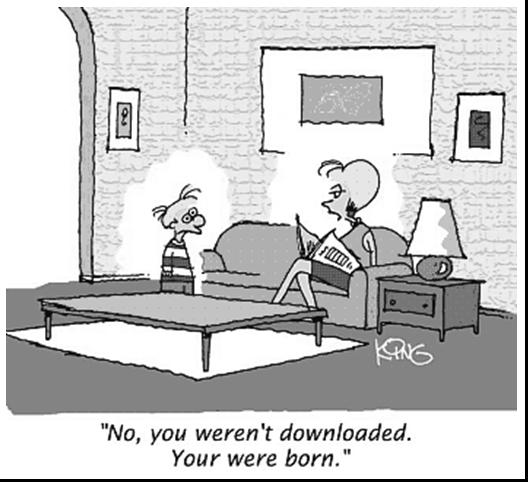
\includegraphics[width=.5\textwidth]{fig1.jpg}
\caption{A typical figure}
\label{fig:exampleFig1}
\end{figure}

\begin{figure}[ht]
\centering
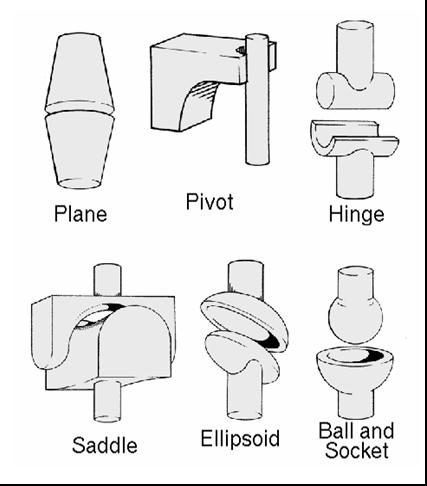
\includegraphics[width=.3\textwidth]{fig2.jpg}
\caption{This figure is an example of a figure caption taking more than one
  line and justified considering margins mentioned in Section~\ref{sec:figs}.}
\label{fig:exampleFig2}
\end{figure}

In tables, try to avoid the use of colored or shaded backgrounds, and avoid
thick, doubled, or unnecessary framing lines. When reporting empirical data,
do not use more decimal digits than warranted by their precision and
reproducibility. Table caption must be placed before the table (see Table 1)
and the font used must also be Helvetica, 10 point, boldface, with 6 points of
space before and after each caption.

\begin{table}[ht]
\centering
\caption{Variables to be considered on the evaluation of interaction
  techniques}
\label{tab:exTable1}
\smallskip
\begin{tabular}{|l|c|c|}
\hline
& Value 1 & Value 2\\[0.5ex]
\hline
&&\\[-2ex]
Case 1 & 1.0 $\pm$ 0.1 & 1.75$\times$10$^{-5}$ $\pm$ 5$\times$10$^{-7}$\\[0.5ex]
\hline
&&\\[-2ex]
Case 2 & 0.003(1) & 100.0\\[0.5ex]
\hline
\end{tabular}
\end{table}

\section{Images}

All images and illustrations should be in black-and-white, or gray tones,
excepting for the papers that will be electronically available (on CD-ROMs,
internet, etc.). The image resolution on paper should be about 600 dpi for
black-and-white images, and 150-300 dpi for grayscale images.  Do not include
images with excessive resolution, as they may take hours to print, without any
visible difference in the result. 

\section{References}

Bibliographic references must be unambiguous and uniform.  We recommend giving
the author names references in brackets, e.g. \cite{knuth:84},
\cite{boulic:91}, and \cite{smith:99}.

The references must be listed using 12 point font size, with 6 points of space
before each reference. The first line of each reference should not be
indented, while the subsequent should be indented by 0.5 cm.

\bibliographystyle{sbc}
\bibliography{sbc-template}

\end{document}
